Project launched in October 2014 by Olivier Georgeon on the internet platform MOOC\footnote{\href{http://liris.cnrs.fr/ideal/mooc/}{\texttt{\scriptsize http://liris.cnrs.fr/ideal/mooc/}}} consisting of learning and developing a new concept in artificial intelligence called IDEAL (\textbf{I}mplementation of \textbf{DE}velopment\textbf{A}l \textbf{L}earning) -- defined as an ``approach to simulate the early mechanisms of emergent cognition based on theories of enactive cognition and on constructivist epistemology'' \citep{ger}.

\begin{wrapfigure}{r}{0.35\textwidth}
%  \vspace{-25pt}
%   \hspace{-5pt} 
\vspace{-5pt}
   \hspace{-5pt} 
   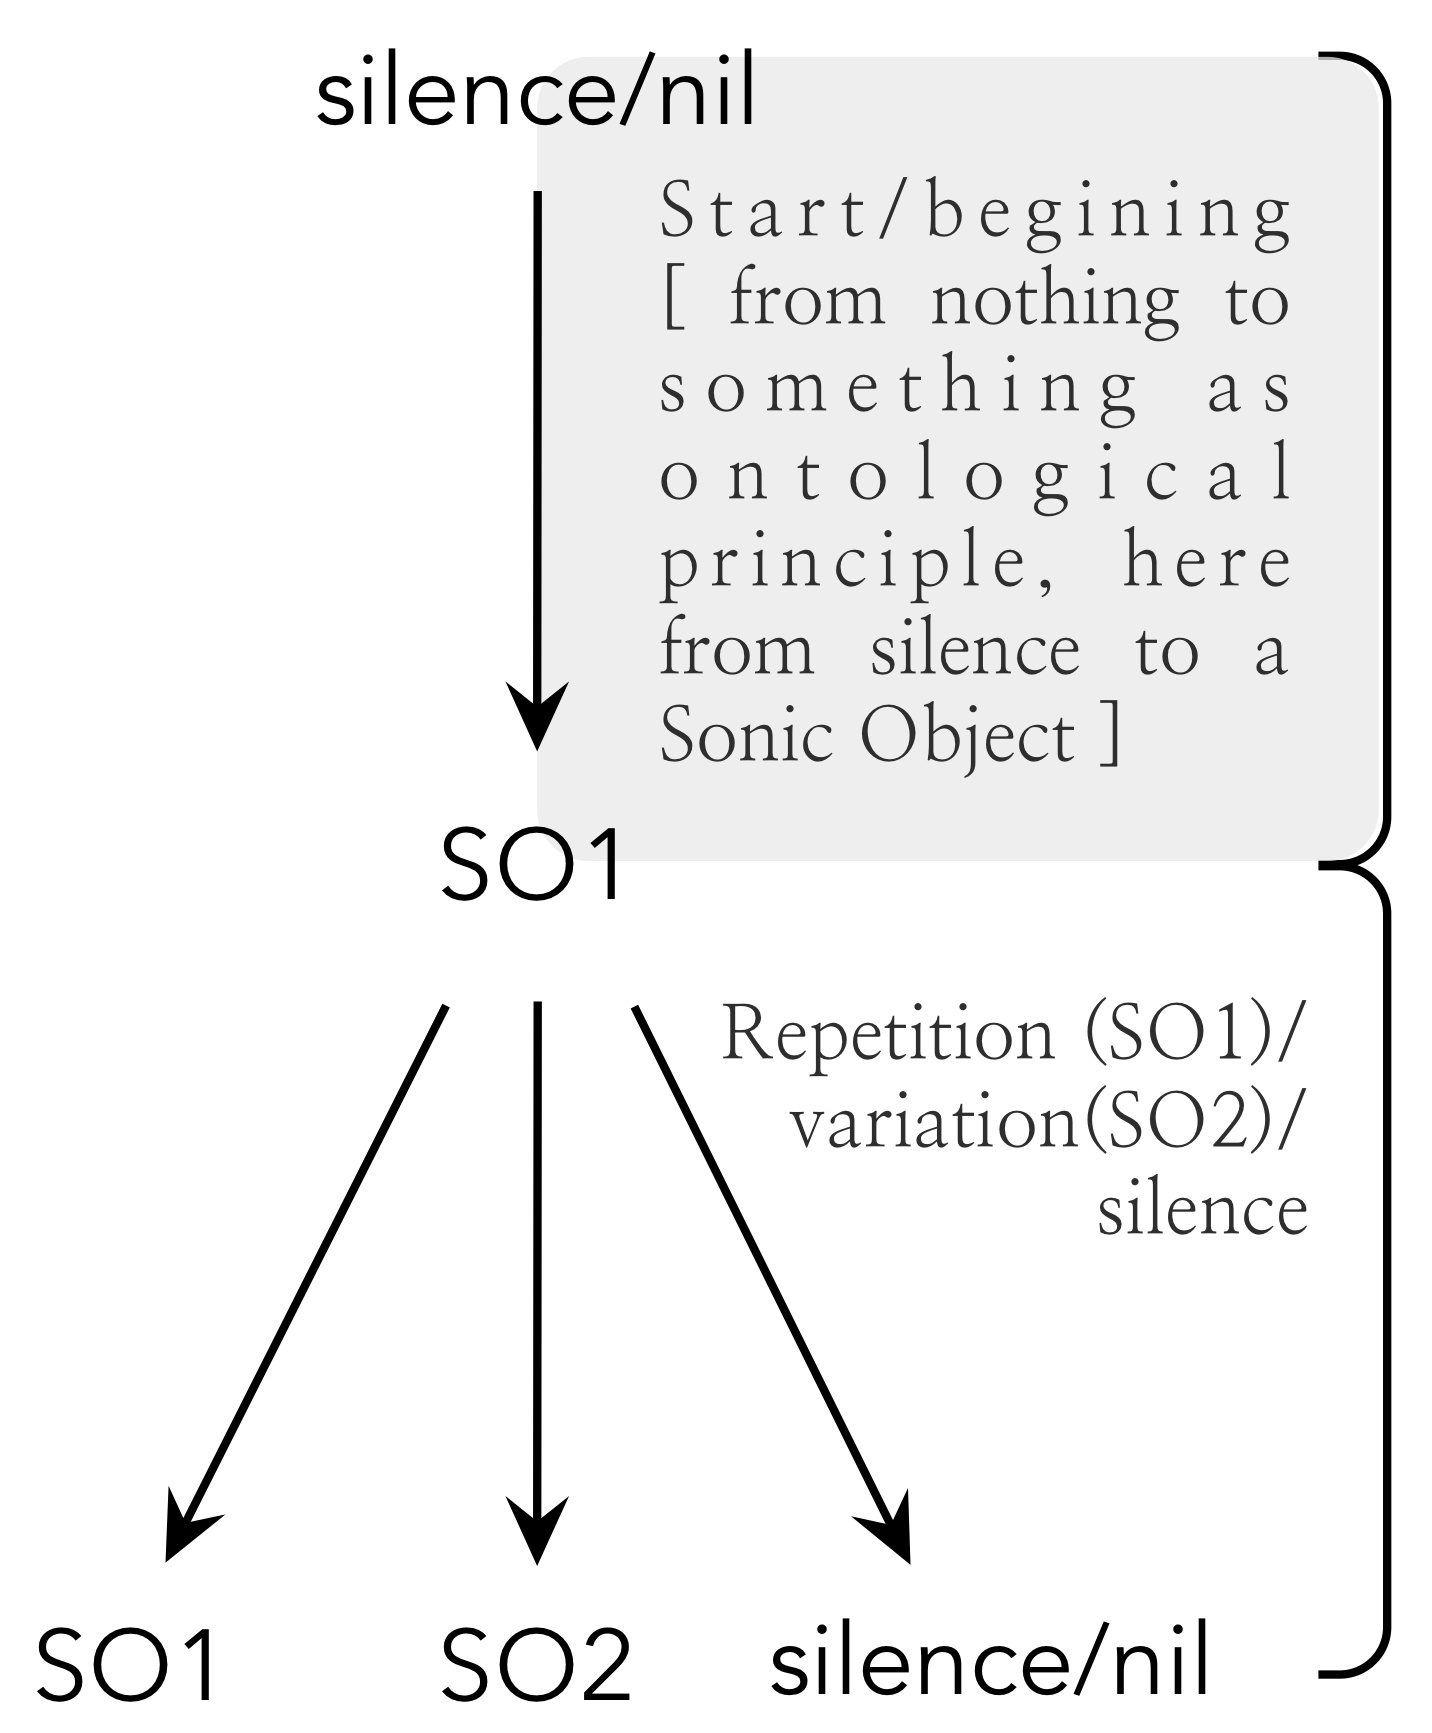
\includegraphics[width=0.35\textwidth]{2345}
  %\caption{...}
  \vspace{-20pt}
\end{wrapfigure}

\bigskip

Then, the idea in the context and in the continuation of \textsl{Neuromuse3}\footnote{\href{https://github.com/yannics/N3D}{\texttt{\scriptsize https://github.com/yannics/N3D}}} is to create a kind of emergent intelligence from the network previously described, composed of cliques and \textit{tournois}, by including additional learning process defined by IDEAL based on the experimentation and on the experience. 

\bigskip

It is opportun to underline the philosophical aspect of this approach in terms of modeling including a causal device as computational cognition.

Thus, each agent develops its own understanding of its environment -- i.e. an ontological conception in epistemological terms.

Also, IDEAL implies non-ontological interactional presuppositions -- the ontological aspect will be defined by the agent as it experiences its interaction with the environment.

\bigskip
\bigskip

\noindent {\large \textbf{Glossary}}

\bigskip

Abbreviations: \textsl{fr.} = French; \textsl{acc.} = \textit{acception}.

\begin{description}
\item[Enaction]: interaction with the environment.
\item[Proclivity]: [\textsl{fr}. \textit{propension}] inner, innate, natural force, which directs spontaneously or voluntarily towards an action, a behavior.
\item[Valence]:  [\textsl{acc.} psychology] refers to the intrinsically pleasant or unpleasant quality of a stimulus or situation.
\end{description}

\bigskip

 \begin{notes}
%Developmental Artificial Intelligence. Lesson 1/4
%
%\href{https://www.youtube.com/watch?v=aQWnx1PX7-w}{\texttt{\scriptsize https://www.youtube.com/watch?v=aQWnx1PX7-w}}

%Developmental Artificial Intelligence. Lesson 2/4
%
%\href{https://www.youtube.com/watch?v=5AnDYmEAF5I}{\texttt{\scriptsize https://www.youtube.com/watch?v=5AnDYmEAF5I}}
%
%Developmental Artificial Intelligence. Lesson 3/4
%
%\href{https://www.youtube.com/watch?v=iM7j2a3pLNk}{\texttt{\scriptsize https://www.youtube.com/watch?v=iM7j2a3pLNk}}
%
%Developmental Artificial Intelligence. Lesson 4/4
%
%\href{https://www.youtube.com/watch?v=v6YXon6Y4iU}{\texttt{\scriptsize https://www.youtube.com/watch?v=v6YXon6Y4iU}}

%\vfill\hfill\smash{\raisebox{5pt}{\includegraphics[width=2cm,height=2cm]{1223}}} 

{\large \textbf{Summary description}}

\begin{description}
\item[\texttt{E010}] 
When the expected or desired result is effective, according to the conditions of \texttt{result010}, the qualitative character self-satisfied is `activated' (frustrated otherwise). After $n$ identical, similar, equivalent or other interactions, this is the bored character that is activated, and the system look for another experience to avoid `boredom'.

\item[\texttt{E020}]
The character is quantified with the valence expressing the motivation. This is applied to the primitive interactions.

\quad -- valence $\geq 0 \Rightarrow$ pleased

\quad -- valence $< 0 \Rightarrow$ pained

\item[\texttt{E030}]
Continuation of \texttt{E020} including composite interactions (indeed first level abstractions).

%[\texttt{E020} and \texttt{E030} could imply a fractal dispersion toward the macroscopic ... i.e. a demonstrable influence in terms of fractality on composite interactions and abstractions.]

\item[\texttt{E031}]
Variation of \texttt{E030} involving weights in terms of proclivity.

%\item[\texttt{E040}]

%Arbre binaire entier et nombre de Catalan
%Un arbre binaire entier est un arbre dont chaque nœud possède zéro ou deux fils.
%Le nombre de Catalan est le nombre d'arbres binaire entier que l'on peut construire avec n éléments.
%Ce nombre est définit par la formule suivante: ...
\end{description}

\end{notes}

\bigskip
\bigskip

\noindent {\large \textbf{Index}}

\bigskip

\begin{description}[font=\ttfamily]

\item[*PROCLIVITY*] \textit{<t/nil>}

\item[*REMANENCE*] \textit{<integer>}

\item[*VERBOSE*] \textit{<t/nil>}

\item[ADD-OR-GET-EXPERIMENT] \textit{<existence>} \textsl{\&key} label \textit{<symbol>} string \textit{<string>}

\item[ADD-OR-GET-INTERACTION] \textit{<existence>} \textit{<experiment/pre-interaction>} \\ \textit{<result/post-interaction>} \textsl{\&key} valence \textit{<number>} learn \textit{<t/nil>}

\item[ADD-OR-GET-RESULT] \textit{<existence>} \textsl{\&key} label \textit{<symbol>} string \textit{<string>}

\item[CREATE-AGENT] \textit{<name>}

\item[GET-PRIMITIVE-EXPERIENCE] \textit{<experiment/interaction>}

\item[PICK-EXPERIMENT] \textit{<existence>}

\item[PICK-OTHER-EXPERIENCE] \textit{<existence>} \textit{<experiment>}

\item[PREDICT] \textit{<existence>} \textit{<experiment/interaction>} \\ From \textit{existence-interactions}, the evaluation is a \textit{result}.

\item[>REMANENCE] \textit{<existence>} \textit{<experiment/interaction>} \\ Update of \textit{existence-previous} by adding an \textit{experiment} or an \textit{interaction} in the MCT (short-term memory) with |MCT| = \texttt{*REMANENCE*}

\item[RUN-AGENT] <\textit{name}> \textsl{\&key} duration \textit{<integer>} step \textit{<function>} \\ result \textit{<function>}

\item[SELECT-ANTICIPATE] \textit{<existence>} \textit{<experiment/interaction/null>} \\ From \textit{existence-interaction}(s), the evaluation is an \textit{interaction}.

\end{description}